\chapter{Evaluation}
\label{cha:eval}
This research project has among its main aims the evaluation of results, described in this chapter. It is important to analyse how this general purpose application performs under the SpiNNaker environments and what architectural limitations it faces, which is useful feedback to the team. The chapter outlines also performance benchmarks of SpiDB in comparison with other database systems and how it can be improved.

\section{Reliability \& transmission rate}
\label{sec:eval_comm_rel}

According to my experiments, sending SDP packets immediately between two cores results on a very large packet drop ration. Without explicit delay/wait between the transmission of packets, the number of successful deliveries is only about 10\% of those sent for a large number of packets. This effect is strongly reduced by the addition of a small delay of 5-10$\mu$s, which guarantees over 99\% successful deliveries, as can be seen on table \ref{table:sdp_deliveries}. The table also shows that long intervals, greater than 10$\mu$s, are mostly redundant, as they do not decrease packet loss significantly, but tragically reduce throughput.

Upon experimenting, I found that sending a large amount of consecutive, immediate packets (at least 1,000,000) has a chance of consequently crashing the destination core or causing it to reach the erroneous watchdog state (WDOG), meaning it cannot respond to commands.

\begin{table}
\begin{tabular}{ r | c | c | c | c | c }
 & \multicolumn{5}{c}{\textbf{Successful deliveries (\%)}} \\

\textbf{Packets sent} & \textbf{no delay} & \textbf{2$\mu$s delay} & \textbf{5$\mu$s delay} & \textbf{10$\mu$s delay} & \textbf{100$\mu$s delay} \\
50,000 & 9.56\% & 57.73\% & 95.95\% & 98.36\% & 99.85\% \\
100,000 & 12.15\% & 54.97\% & 97.99\% & 99.13\% & 99.92\% \\
200,000 & 13.07\% & 50.55\% & 99.01\% & 99.33\% & 99.96\% \\
500,000 & 12.97\% & 50.08\% & 99.49\% & 99.80\% & 99.99\% \\
1,000,000 & 13.05\% & 45.06\% & 98.84\% & 99.88\% & 99.99\% \\
\end{tabular}
\caption{Successful SDP deliveries with delay between each packet}
\label{table:sdp_deliveries}
\end{table}

Note that the experiment, made on SpiNN-3, involved sending a single SDP packet multiple times to the same destination on the same chip, containing only the 8 byte SDP header. The destination did not store or read the packet contents, only incrementing a counter upon packet receival. This was used to show the maximum possible transmission rate allowed by the SDP protocol under the hardware communication fabric. Code snippets and more information can be found on the appendix under the appendix section \ref{sec:appendix_comm_rel}.

Ideally these packets would send useful information, to be read upon arrival, which would keep the destination busy. From my experience and input from the team, the best way to achieve this is by immediately storing the SDP packet contents into a buffer when it is received and then handling it at a different point in time (listing \ref{lst:sdp_packet_callback} under appendix). The reason for this is that if another packet arrives as we are processing the current packet with same or higher priority, the incoming packet will drop.

High priority should be assigned to storing incoming packets into a buffer and the actual processing should have lower priority, as it can be handled at a later point in time. It is important to note that this can cause starvation and buffer overflow if there are too many immediate packets being received. For instance, if our SDP packet is of size 12-byte (8-byte header + 32-bit data) and stored into a buffer in private DTCM memory upon receival, we would only ever be able to hold up to about 5,000 messages at once (64-Kbytes DTCM size / 12-byte packet size). Realistically a large part of DTCM contains the stack, local and global variables, so that number will be drastically reduced. In my application, SpiDB, insert and retrieve database queries have a size of 256-bytes, which means a limit of 250 entries in the buffer if memory were empty.

\begin{figure}
\begin{center}
	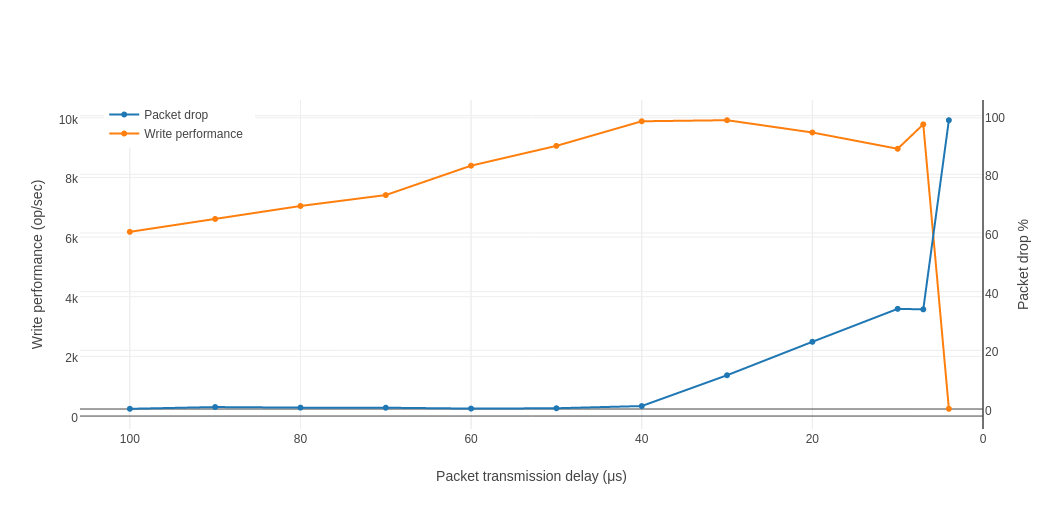
\includegraphics[width=1.3\textwidth, natwidth=1063, natheight=509]{images/transmission_delay.png}
\end{center}
\caption{PUT performance with variable delay}
\label{fig:transmission-delay}
\end{figure}
	
A measured test, transmitting data from a host machine to an Ethernet attached SpiNNaker chip and then to an Application Processor on that node via shared memory, achieved speeds in excess of 22 Mb/s \cite{scalablecomm}.

This evaluation is important because it allows finding the optimal transmission delay and latency for an application. A developer on SpiNNaker using the SDP protocol, which is experimental and yet to be optimised \cite{scalablecomm}, needs to find the balance between transmission rate and reliability, which are inversely proportional.

On SpiDB, I experimented with different time delays when transmitting packets from host over Ethernet to a core on SpiNNaker, in order to find the best evaluation. The speed of one operation is calculated as the time of successful reply minus the time that operation was sent from host, thus being a round-trip-time plus internal processing time. The performance is calculated as the amount of operations successfully executed in one second.

Figure \ref{fig:transmission-delay} plots the performance (left Y axis) and packet drop percentage (right Y axis) of PUT operations  with the decrease of transmission delay. As can be seen, large packet transmission delays of 50-100$\mu$s are redundant, as they do not reduce packet drops, while being a high cost on performance. Naturally the more packets we can send in one second influences the speed of replies, thus improving performance. This hits a maximum at 40$\mu$s, with almost 10,000 op/sec, in which transmission is at a high rate with no loss of reliability. Transmission delays between 40-10$\mu$s result on a decrease of performance, because although packets are sent more frequently, a lot of them are dropped (up to about 35\%), being also extremely unreliable. Naturally performance of is inversely proportional to packet drop rate, as unsuccessful queries do not contribute to the final result. We reach the worst case at 10-5$\mu$s delay, when the destination core cannot cope with the speed of incoming packets, simply crashing and ceasing to respond. A very similar behaviour is visible for \textit{pull} operations, as plotted on figure \ref{fig:hash-performance}.

These SpiDB experiments were performed with 100,000 \textit{put} operations with keys and values of size 4-bytes each. More information on the data gathered for these experiments can be found on the appendix under section \ref{sec:appendix_comm_rel}.

\begin{figure}
\begin{center}
	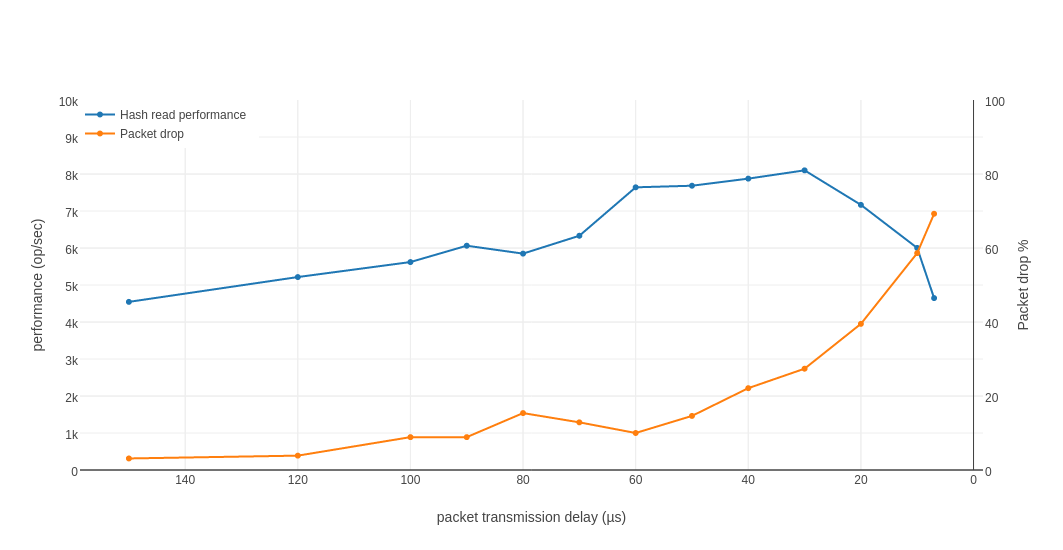
\includegraphics[width=1.3\textwidth, natwidth=1063, natheight=550]{images/hash_performance.png}
\end{center}
\caption{HASH PULL performance with variable delay}
\label{fig:hash-performance}
\end{figure}

These results are largely influenced by the latency of the SDP datagram, driving the need of such delays. A simulation framework described by Navaridas et al. \cite{impacttraffic} has shown how latency scales with system size by simulating a range of system configurations from 16 × 16 (256 nodes) to 256 × 256 (65,536 nodes) on SpiNNaker. The average and maximum latencies obtained after a simulation of 100,000 cycles are plotted in figure \ref{fig:latency} \cite{scalablecomm}. End-to-end latency scales linearly with the number of nodes, i.e. $O(N)$. The maximum latency is that needed to reach the most distant nodes. This means when designing a SpiNNaker application, a developer needs to take into account the locality of communications and the expected latency, which can be used to determine transmission rates.

\begin{figure}
\begin{center}
	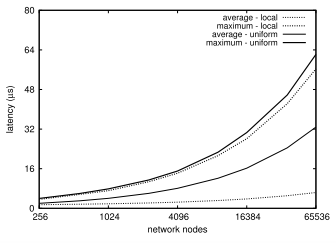
\includegraphics[width=.7\textwidth, natwidth=336, natheight=243]{images/latency.png}
\end{center}
\caption{Latency scalability under uniform and local traffic distributions \cite{scalablecomm}}
\smallskip

\caption*{\footnotesize 
\setlength{\leftskip}{1.5cm}
\setlength{\rightskip}{1.5cm}
Local distribution emulates close proximity destinations. Traffic following a uniform distribution represents a very pessimistic scenario in which locality is not exploited.}

\label{fig:latency}
\end{figure}

%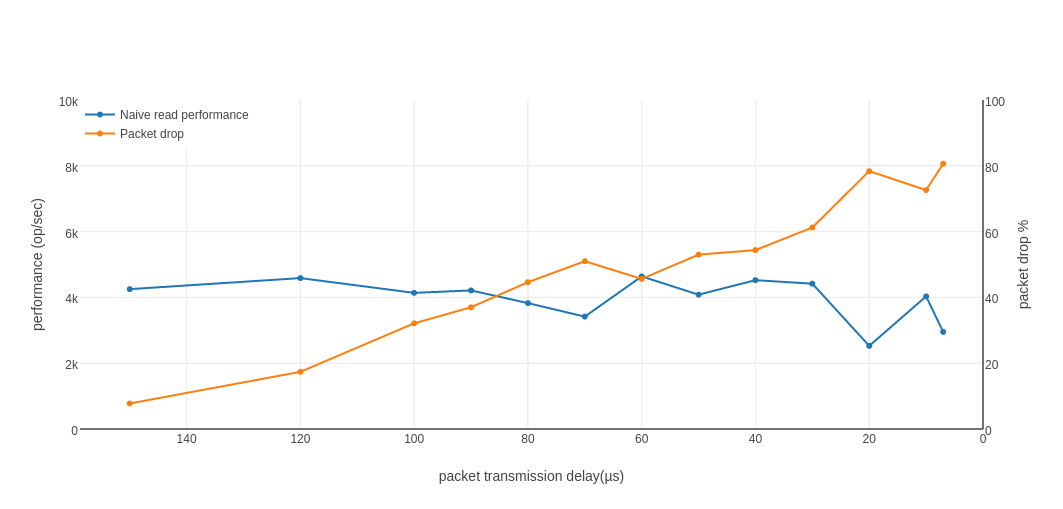
\includegraphics[width=1\textwidth, natwidth=1063, natheight=509]{images/naive_performance.png}

%what are reasons for packets to drop? because thingy just takes 1 microsecond or does it?...

\section{Performance benchmark}
In order to evaluate the performance of my Key-Value database management system, I compared it with two of the most popular RAM-based Key-Value pair databases: \textbf{Memcached} \cite{memcached} and \textbf{Redis} \cite{redis}. NoSQL databases have recently become particularly popular \cite{nosqlsurvey} and these two systems have been on the market for multiple years, thus serving as a good comparison to my project, SpiDB.

Figure \ref{fig:write-perf-benchmark} shows a performance plot of the SpiNNaker Database (SpiDB) against these competitors for 100,000 consecutive \textit{put} operations. It can be seen that SpiDB runs at about 7,000-8,000 operations per second, which is slower than the others by a factor of 8. Performance for all systems was mostly constant given input size, up to the maximum SDP data size of 256-bytes. More specification and data gathered can be found at appendix under section \ref{sec:appendix-specs}.

\begin{figure}
\begin{center}
	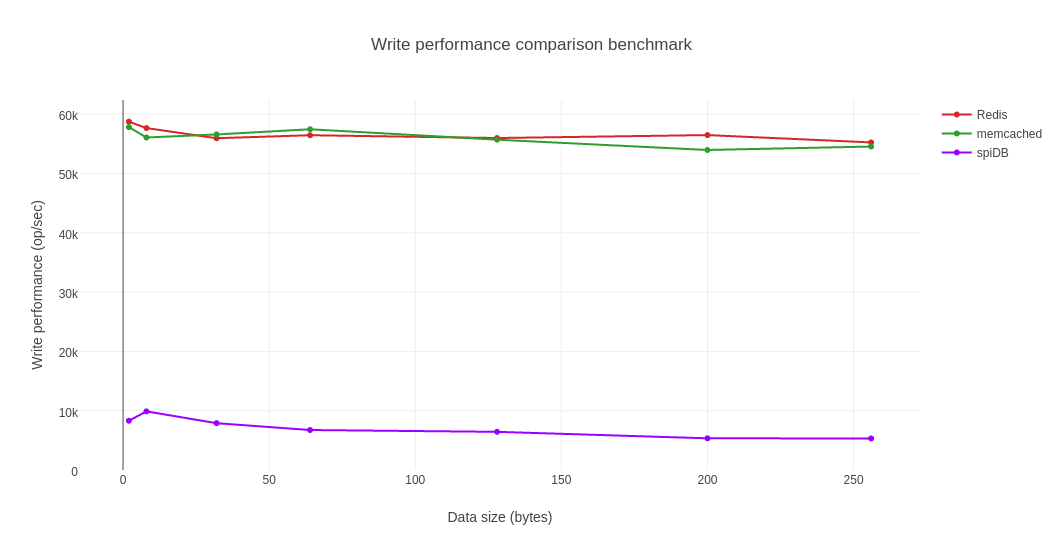
\includegraphics[width=1.4\textwidth, natwidth=1063, natheight=509]{images/write_performance.png}
\end{center}
\caption{PUT operation performance benchmark}
\label{fig:write-perf-benchmark}
\end{figure}

The current SpiDB implementation is new and can be highly enhanced with modifications to the network communication and the addition of caching, which increases the overall performance, enhancing the application in comparison to the other systems. Nevertheless there is a limit to how much improvement can be brought using the SDP protocol, as it has a network and memory bottleneck, earlier discussed in sections \ref{sec:eval_comm_rel} and \ref{sec:limitations}. This means improvements to the code would never allow it to reach performances above around 10,000 operations per second, which is still very slow in comparison with the others.

Another weakness to the approach is the fact that the \textit{root} core is a central point of failure, penalising performance. As of now the SpiNNaker hardware can only host one IP server, at a single chip, to communicate over Ethernet to \textit{host}, meaning incoming and outgoing queries must pass through it. One solution to this is using another external connection, present on SpiNN-4 machines, named \textit{spinnlink}, which allows distributed data transfers.

Although from an initial evaluation it may seem that SpiNNaker is not capable of hosting a database efficiently, that can be proven wrong. It must be outlined that this performance cap is the limitation of a single, independent SpiNNaker board. The SpiNNaker hardware was designed to be inter-connected, allowing transfers of data between boards, which can be used to add another degree of scalability. This means multiple boards can be connected to the host/user and process a set of separate queries in a fully parallel way. Ideally this would result in a linear performance increase proportional to the number of boards connected, meaning that two boards will run the database operations twice faster than one board alone and so forth. From this analysis I can state that an instance of SpiDB running on 8-10 different 4-chip boards will perform better than \textit{Redis} or \textit{memcached} on commercial hardware. The SpiNNaker hardware is expensive to produce for now, but with a decrease on its prices in the future, it can be a very strong candidate for hosting a DBMS.

This scalability work has not yet been fully tested, thus it may serve as constructive speculation for now. It should also be noted that realistically a perfectly linear performance increase with the increase of horsepower is not common, as other factors need to be taken into account, such as synchronisation, fault tolerance, etc.

%response times. why are they so high sometimes?!?!

\section{SDRAM bandwidth utilisation}
\label{sec:limitations}
As discussed in section \ref{sec:spinn_arch}, a single SpiNNaker chip contains 18 cores sharing 128-MB of dynamic memory (SDRAM), used to store/retrieve data and transfer certain packets between cores. An important stage of the design of a SpiNNaker application is managing the share of available resources, such as SDRAM, to maximise collective utilisation and performance.

\begin{figure}
\begin{center}
	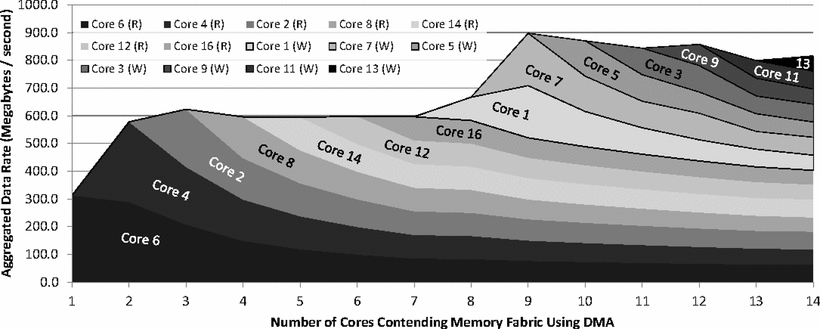
\includegraphics[width=1.3\textwidth, natwidth=820, natheight=329]{images/sdram_bandwidth.png}
\end{center}
\caption{SDRAM bandwidth utilisation \cite{painkras}}
\label{fig:sdram_bandwidth}
\end{figure}

In order to find an efficient way to collectively access SDRAM, its bandwidth has to be taken into account. Figure \ref{fig:sdram_bandwidth}, plotted by E. Painkras et al. \cite{painkras}, shows the aggregate SDRAM bandwidth utilisation of a number of cores on a single SpiNNaker chip, increased progressively from 1 to 14. The plot outlines the DMA transfer rate for each core as they simultaneously access the shared resource \cite{multicoresystem}. It is clear from the figure that the read channel saturates just over 600 MB/s and the write channel adds around 300 MB/s on top of that, for a total aggregate bandwidth of 900 MB/s. Because memory reads and writes share the same network channel, an increase in the number of writes decreases the read bandwidth. Memory bandwidth, although saturated, is distributed fairly among all cores \cite{painkras}. 

The progression of Core 6 on the plot shows that if the DMA controller is free, a single core can read from shared memory at 300 MB/s, but if such memory is being constantly accessed by other processors, each will only retrieve data at a rate of around 50 MB/s (6 times slower than doing so exclusively). This evaluation is important because it shows the limitation of all cores frequently accessing shared memory simultaneously, which is exactly the case of the SpiDB \textit{pull} and \textit{SELECT} queries.

It is worth noting that the core's private memory (DTCM), although 2000 times smaller than SDRAM (64-KB vs 128-MB), is 50 times faster to access and does not suffer from concurrent access limitations, which makes it a strong candidate for the implementation of a \textit{cache} memory. This has not been yet implemented, but with appropriate synchronisation it would highly reduce SDRAM access and reduce response times. On SpiDB another enhancement to minimise unnecessary SDRAM access is the use of a hash-table structure, in which the location of values inserted on the database is always known, avoiding a linear scan through the system.
